\documentclass[12pt,a4paper]{article}

% ---- Paquetes ----
\usepackage[utf8]{inputenc}
\usepackage[spanish]{babel}
\usepackage[T1]{fontenc}
\usepackage{graphicx}
\usepackage{hyperref}
\usepackage{amsmath}
\usepackage{amssymb}
\usepackage{listings}
\usepackage{xcolor}
\usepackage{geometry}
\usepackage{tabularx}
\usepackage{booktabs}
\usepackage{caption}
\usepackage{subcaption}
\usepackage{enumitem}
\usepackage{parskip}
\usepackage{alltt}
\usepackage{float}
\usepackage{pifont}
\usepackage{ragged2e}
\newcolumntype{L}{>{\RaggedRight\arraybackslash}X}

\geometry{margin=2.5cm}
\setlength{\parindent}{0pt}
\setlength{\emergencystretch}{2em}

% ---- Configuración de listings ----
\lstset{
    basicstyle=\ttfamily\small,
    breaklines=true,
    frame=single,
    numbers=left,
    numberstyle=\tiny,
    language=Python,
    keywordstyle=\color{blue},
    commentstyle=\color{gray},
    stringstyle=\color{red},
    tabsize=4,
}

% ---- Hipervínculos ----
\hypersetup{
    colorlinks=true,
    linkcolor=blue,
    urlcolor=blue,
    citecolor=blue,
}

% ---- Comandos CML-DEVS ----
\newcommand{\cmlgt}{$>$}
\newcommand{\cmlle}{$\leq$}
\newcommand{\cmleq}{$=$}
\newcommand{\cmlplus}{$+$}
\newcommand{\cmlN}{$\mathbb{N}$}
\newcommand{\cmlgeq}{$\geq$}
\newcommand{\cmllt}{$<$}
\newcommand{\cmlwedge}{$\wedge$}
\newcommand{\cmlneq}{$\neq$}
\newcommand{\cmlvee}{$\vee$}
\newcommand{\kw}[1]{\textbf{#1}}
\newcommand{\cmlR}{$\mathbb{R}$}
\newcommand{\cmlTime}{\textbf{Time}}
\newcommand{\cmlsigma}{$\sigma$}
\newcommand{\dint}{$\delta_{\mathit{int}}$}
\newcommand{\dext}{$\delta_{\mathit{ext}}$}
\newcommand{\clambda}{$\lambda$}
\newcommand{\cmlta}{\textbf{ta}}
\newcommand{\cmlcomment}[1]{\textit{\textcolor{gray}{#1}}}

\newenvironment{cmldevs}{%
  \begin{alltt}\small%
}{%
  \end{alltt}%
}

% ---- Portada ----
\begin{document}

\begin{titlepage}
    \centering
    \vspace*{3cm}
    
    {\Huge \textbf{Simulador DEVS de una Bomba de Infusión Intravenosa}}
    
    \vspace{1.5cm}
    
    {\Large Trabajo Práctico Integrador}
    
    \vspace{1cm}
    
    {\large \textbf{Materia:} Simulación}
    
    \vspace{0.5cm}
    
    {\large \textbf{Universidad Nacional de Río Cuarto}}
    
    \vspace{2cm}
    
    \textbf{Autores:}
    
    \vspace{0.3cm}
    
    \begin{tabular}{c}
        Hernán Jara \\
        Jhonatan Calle
    \end{tabular}
    
    \vspace{1cm}
    
    {\large 2026}
    
    \vfill
\end{titlepage}

\newpage

% ---- Índice ----
\tableofcontents
\newpage

% ===================================================================
\section{Introducción}
% ===================================================================

\subsection{Contexto}

Una bomba de infusión intravenosa es un dispositivo médico que suministra
fluidos, medicamentos o nutrientes de forma controlada al torrente sanguíneo
del paciente.  Su correcto funcionamiento es crítico para la seguridad del
paciente: un caudal incorrecto puede provocar desde una dosificación
insuficiente hasta una sobredosis letal.

La simulación basada en el formalismo DEVS (\textit{Discrete Event System
Specification}) permite modelar el comportamiento discreto del sistema de
control de la bomba, verificar propiedades de seguridad y liveness, y
analizar el impacto de fallas en los componentes antes de la implementación
física.

\subsection{Objetivo}

El objetivo de este trabajo es:

\begin{itemize}
    \item Modelar el sistema de control de una bomba de infusión
          intravenosa simplificada utilizando el formalismo DEVS.
    \item Implementar el modelo en Python utilizando el motor de
          simulación PyPDEVS.
    \item Definir y verificar un conjunto de propiedades de safety,
          liveness y temporalidad sobre el comportamiento del sistema.
    \item Evaluar el sistema frente a distintos escenarios de
          funcionamiento normal y de falla, incluyendo desvíos de caudal,
          fin de bolsa, alarmas críticas y una violación deliberada de
          seguridad.
    \item Generar gráficos y reportes cuantitativos que permitan
          analizar el comportamiento del sistema.
    \item Proponer mejoras para reducir riesgos en el controlador.
\end{itemize}

\subsection{Alcance}

El sistema modelado comprende siete modelos atómicos:

\texttt{GeneradorOrdenes}, \texttt{SensorFlujo}, \texttt{ActuadorBomba},
\texttt{ControladorBomba}, \texttt{ModuloAlarmas},
\texttt{GeneradorConfirmacion} y \texttt{GeneradorFinBolsa},
interconectados en un modelo acoplado.

Se definieron 8 escenarios determinísticos y estocásticos que cubren
operación normal, cambios de orden, desvíos de caudal, fin de bolsa y
alarmas críticas, más un escenario adicional (escenario 9) que introduce
una violación deliberada de seguridad para demostrar la capacidad del
verificador de detectar comportamientos inseguros.

La verificación consta de 10 propiedades (P1--P10) que abarcan safety,
liveness y restricciones temporales.  Adicionalmente, se genera un
reporte de resultados con métricas cuantitativas (alarmas generadas,
tiempos de respuesta, detenciones preventivas y porcentaje de tiempo
con infusión correcta) y gráficos de caudal, estado de la bomba y
timeline de eventos.

\subsection{Estructura del documento}

El resto del documento se organiza de la siguiente manera:

\begin{description}[leftmargin=2.5cm, style=nextline]
    \item[Sección 2:] describe el sistema y sus componentes.
    \item[Sección 3:] presenta la especificación formal DEVS de cada
          modelo atómico y del modelo acoplado.
    \item[Sección 4:] detalla la implementación en PyPDEVS y la
          infraestructura de validación.
    \item[Sección 5:] presenta los escenarios de simulación, los
          resultados obtenidos y el análisis visual.
    \item[Sección 6:] propone mejoras para reducir riesgos en el
          controlador.
    \item[Sección 7:] expone las conclusiones del trabajo.
\end{description}

% ===================================================================
\section{Descripción del Sistema}
% ===================================================================

\subsection{Visión general}

El sistema modela el comportamiento de una bomba de infusión intravenosa
simplificada, encargada de administrar una droga a un paciente respetando
una dosis objetivo indicada por una orden médica.  El sistema completo se
compone de siete modelos atómicos DEVS que se comunican mediante puertos
de entrada y salida, formando un modelo acoplado que reproduce tanto el
funcionamiento normal del equipo como sus mecanismos de seguridad ante
fallas.

El comportamiento se centra en tres ejes:
\begin{enumerate}
    \item la administración del caudal indicado dentro de los tiempos de
          respuesta exigidos;
    \item la detección y escalado de desvíos sostenidos en el caudal real
          respecto del objetivo;
    \item la reacción ante el agotamiento de la bolsa de medicación.
\end{enumerate}
Todo ello acompañado de un esquema de alarmas que notifica al personal
médico y exige su intervención en los casos más críticos.

\subsection{Componentes del sistema}

A continuación se describen los siete modelos atómicos que componen el
sistema.

\subsubsection{Generador de Órdenes Médicas}
\texttt{GeneradorOrdenes} es un modelo autónomo (sin puertos de entrada)
que produce periódicamente eventos \texttt{ordenMedica} indicando el
caudal objetivo (entre 0 y 200 ml/h) que la bomba debe administrar.  Una
orden con caudal igual a cero indica la detención de la infusión.  El
generador puede operar en modo determinístico (caudal e interarribo fijos)
o estocástico (caudal según distribución Normal, interarribo según
distribución Exponencial).

\subsubsection{Generador de Fin de Bolsa}
\texttt{GeneradorFinBolsa} es un modelo autónomo que genera el evento
\texttt{finBolsa} una única vez cuando la bolsa de medicación está
próxima a agotarse.  Puede configurarse con un tiempo fijo determinístico
o con una distribución Normal para simular variabilidad en el
agotamiento del reservorio.

\subsubsection{Generador de Confirmación de Enfermero}
\texttt{GeneradorConfirmacion} es un modelo autónomo que genera
periódicamente el evento \texttt{confirmacionEnfermero}, simulando el
reconocimiento manual de alarmas por parte del personal médico.  Opera
con un límite máximo de confirmaciones; puede configurarse con un tiempo
fijo o con una distribución Log-Normal.  La confirmación permite salir
del estado de alarma crítica y reanudar la operación.

\subsubsection{Sensor de Flujo}
\texttt{SensorFlujo} mide e informa el caudal real administrado cada
1 segundo exacto.  Recibe del actuador el valor físico real
(\texttt{caudalActual}) y lo incorpora en su próxima medición.  Modela
además una deriva temporal: cuanto más tiempo pasa sin una actualización
del actuador, mayor es la posible discrepancia entre el valor reportado
y el valor base, según la tasa \texttt{TASA\_DERIVA\_SENSOR = 2\%}
del caudal por segundo.  Opcionalmente puede agregar ruido gaussiano a
la medición.

\subsubsection{Actuador de la Bomba}
\texttt{ActuadorBomba} representa el mecanismo físico que administra la
medicación.  Recibe del controlador las órdenes \texttt{ajustarCaudal} y
\texttt{detenerBomba}, y aplica el cambio físico tras una latencia fija
de 0.5 segundos, notificando luego el nuevo caudal real al sensor mediante
\texttt{caudalActual}.  Puede configurarse con un \texttt{factor\_falla}
que reduce el caudal real respecto del comandado, simulando desperfectos
mecánicos (por ejemplo, \texttt{factor\_falla = 0.80} produce un desvío
permanente del 20\%).

\subsubsection{Módulo de Alarmas}
\texttt{ModuloAlarmas} gestiona las notificaciones hacia el personal
médico a través del puerto \texttt{alarma} (con valores \texttt{baja},
\texttt{media}, \texttt{critica}).  Tras notificar una alarma crítica,
espera 30 segundos por una confirmación del enfermero; si no llega,
repite la notificación cada 10 segundos de forma indefinida hasta ser
confirmada.  Las alarmas baja y media son de notificación única.
El módulo incluye un guarda que ignora eventos \texttt{CRITICA}
adicionales mientras ya está manejando una, preservando el primer
timer de 30 segundos.

\subsubsection{Controlador de Bomba}
\texttt{ControladorBomba} es el componente central del sistema.  Recibe
las cuatro entradas externas (\texttt{ordenMedica}, \texttt{sensorFlujo},
\texttt{finBolsa}, \texttt{confirmacionEnfermero}) y decide las acciones
de control: ajustar el caudal, detener la bomba, o emitir una alarma.
Mantiene internamente la máquina de estados de la infusión con las
siguientes fases:

\begin{itemize}
    \item \texttt{OCIOSO} --- bomba detenida, sin infusión activa.
    \item \texttt{INFUNDIENDO} --- infusión en curso, caudal objetivo
          activo.
    \item \texttt{ALERTA\_BOLSA} --- fin de bolsa detectado, se permite
          hasta 60 segundos adicionales de infusión.
    \item \texttt{ALARMA\_MEDIA} --- desvío sostenido por más de 5
          segundos; primera advertencia.
    \item \texttt{ALARMA\_CRITICA} --- según el criterio propio del
          equipo (dos episodios de alarma media sin corrección); se
          detiene la bomba y se exige confirmación.
    \item \texttt{PARADA\_POR\_BOLSA} --- tiempo máximo tras fin de bolsa
          agotado; la bomba se detiene automáticamente.
\end{itemize}

El controlador gestiona temporizadores independientes para el desvío
de caudal (\texttt{t\_desvio}) y el fin de bolsa (\texttt{t\_bolsa}),
ambos manejados de forma concurrente mediante la función
\texttt{\_sigma\_min()} que devuelve el mínimo de los timers
activos.  Al recibir una orden médica, programa una demora de 2
segundos antes de emitir \texttt{ajustarCaudal}.  Cuando detecta el
primer desvío, emite un ajuste inmediato (\texttt{sigma = 0.0}) e
inicia un timer de 5 segundos.  En desvío sostenido, el sigma
resultante combina el tiempo restante de los timers activos mediante
\texttt{min(sigma\_restante,}\penalty0\relax
\texttt{\_sigma\_min(t\_desvio,}\penalty0\relax
\texttt{t\_bolsa))},
preservando el timer pendiente de la orden médica.

El controlador incluye además un guarda configurable
(\texttt{violar\_seguridad}) que permite ignorar las lecturas del
sensor durante la fase \texttt{ALARMA\_CRITICA} y reinicia la fase a
\texttt{INFUNDIENDO}.
Esto se utiliza en el escenario 9 para demostrar la detección de
violaciones de seguridad.

\subsection{Modelo acoplado}

Los siete modelos atómicos se integran en el modelo acoplado
\texttt{SistemaBomba}, que define las conexiones internas y los puertos
de salida observables desde el exterior.  Las conexiones son las
siguientes:

Con \texttt{GeneradorOrdenes} enviando órdenes al controlador:
\[\texttt{ordenMedica} \to \texttt{ControladorBomba}\]
El controlador comanda al actuador:
\[\texttt{ajustarCaudal} \to \texttt{ActuadorBomba},\qquad
\texttt{detenerBomba} \to \texttt{ActuadorBomba}\]
El actuador informa al sensor:
\[\texttt{caudalActual} \to \texttt{SensorFlujo}\]
El sensor retroalimenta al controlador:
\[\texttt{sensorFlujo} \to \texttt{ControladorBomba}\]
El generador de fin de bolsa notifica al controlador:
\[\texttt{finBolsa} \to \texttt{ControladorBomba}\]
La confirmación del enfermero llega tanto al controlador como
al módulo de alarmas:
\[\texttt{confirmacionEnfermero} \to \texttt{ControladorBomba}\]
\[\texttt{confirmacionEnfermero} \to \texttt{ModuloAlarmas}\]
Finalmente, el controlador envía alarmas al módulo de alarmas:
\[\texttt{alarma} \to \texttt{ModuloAlarmas}\]

Los puertos de salida externos del modelo acoplado son:

\begin{itemize}
    \item \texttt{caudalActual} --- caudal físico real (del
          \texttt{ActuadorBomba}).
    \item \texttt{registrarEvento} --- log de auditoría (del
          \texttt{ControladorBomba}).
    \item \texttt{notificacionAlarma} --- mensajes de alarma (del
          \texttt{ModuloAlarmas}).
\end{itemize}

\subsection{Parámetros del sistema}

La \texttt{config.py} define las constantes del sistema que se listan
en la Tabla~\ref{tab:parametros}.

\begin{table}[ht]
    \centering
    \caption{Parámetros del sistema}
    \label{tab:parametros}
    \begin{tabularx}{\textwidth}{LcL}
        \toprule
        \textbf{Parámetro} & \textbf{Valor} & \textbf{Descripción} \\
        \midrule
        \texttt{PERIODO\_SENSOR} & 1.0 s & Período de muestreo del sensor \\
        \texttt{LATENCIA\_ACTUADOR} & 0.5 s & Latencia física del actuador \\
        \texttt{DESVIO\_MAX\_PERMITIDO} & 10\% & Desvío máximo tolerado \\
        \texttt{TIEMPO\_MAX\_DESVIO} & 5.0 s & Tiempo máx. con desvío antes de alarma \\
        \texttt{TIEMPO\_CONF\_CRITICA} & 30.0 s & Ventana para confirmar alarma crítica \\
        \texttt{PERIODO\_REP\_CRITICA} & 10.0 s & Período de repetición de alarma crítica \\
        \texttt{TIEMPO\_MAX\_FIN\_BOLSA} & 60.0 s & Tiempo máx. tras fin de bolsa \\
        \texttt{CAUDAL\_MIN} & 0.0 ml/h & Caudal mínimo \\
        \texttt{CAUDAL\_MAX} & 200.0 ml/h & Caudal máximo \\
        \texttt{TIEMPO\_INICIO\_INFUSION} & 3.0 s & Tiempo máx. para iniciar infusión tras orden \\
        \texttt{TASA\_DERIVA\_SENSOR} & 2\%/s & Deriva del sensor por segundo sin corrección \\
        \bottomrule
    \end{tabularx}
\end{table}

Además, los parámetros estocásticos incluyen la media y desviación
estándar del fin de bolsa (Normal), los parámetros mu y sigma de la
confirmación (Log-Normal), y la media y desvío del caudal e interarribo
de las órdenes (Normal y Exponencial respectivamente).  Todos los
generadores estocásticos utilizan la semilla 42 para garantizar
reproducibilidad.

% ===================================================================
\section{Especificación Formal DEVS}
% ===================================================================

A continuación se presenta la especificación formal de cada modelo
atómico utilizando el lenguaje CML-DEVS.  Cada
especificación define el conjunto de estados ($S$), los puertos de
entrada ($X$) y salida ($Y$), la función de transición interna
($\delta_{\mathit{int}}$), la función de transición externa
($\delta_{\mathit{ext}}$), la función de salida ($\lambda$) y la
función de avance temporal ($ta$).

% ----------------------------------------------------------------
\subsection{Generador de Órdenes Médicas}

El modelo \textbf{GeneradorOrdenes} es un modelo atómico autónomo (sin
entradas) que genera periódicamente eventos \texttt{ordenMedica},
indicando el caudal objetivo que debe administrar la bomba.  Las
órdenes pueden generarse de manera determinística (caudal y tiempo
entre órdenes fijos) o estocástica (caudal con distribución gaussiana,
interarribo con distribución exponencial) según los escenarios
definidos en \texttt{config.py}.

\begin{center}
\begin{cmldevs}
\kw{atomic} GeneradorOrdenes \kw{is} <Y, S, \dint{}, \clambda{}, \cmlta{}> \kw{where}
\kw{S is}
    caudalProximo : \cmlR{};    \cmlcomment{-- caudal objetivo (0 a 200 ml/h)}
    interarribo   : \cmlTime{};  \cmlcomment{-- tiempo hasta la siguiente orden}
    \cmlsigma{}             : \cmlTime{};  \cmlcomment{-- variable de avance de tiempo}
\kw{end S}
\kw{Y is}
    ordenMedica : \cmlR{};      \cmlcomment{-- puerto de salida: valor del caudal}
\kw{end Y}
\dint{}(caudalProximo, interarribo, \cmlsigma{}) \kw{is}
    \cmlcomment{-- Determinístico: valores fijos del config}
    \cmlcomment{-- Estocástico: caudal ~ Gauss(media, desvío), interarribo ~ Exp(media)}
    caudalProximo = next\_caudal\_logic();
    interarribo   = next\_interarribo\_logic();
    \cmlsigma{}   = interarribo;
\kw{end} \dint{}
\clambda{}(caudalProximo, interarribo, \cmlsigma{}) \kw{is}
    ordenMedica = caudalProximo;
\kw{end} \clambda{}
\cmlta{}(caudalProximo, interarribo, \cmlsigma{}) \kw{is}
    \cmlsigma{};
\kw{end} \cmlta{}
\kw{end atomic}
\end{cmldevs}
\captionof{figure}{Especificación CML-DEVS: Generador de Órdenes Médicas}
\label{fig:generador-ordenes}
\end{center}

\subsubsection*{Análisis del modelo}

\begin{enumerate}
    \item \textbf{Modos de generación}: En modo determinístico,
    los valores \texttt{caudal\_fijo} e \texttt{interarribo\_fijo}
    provienen del \texttt{config.py}.  En modo estocástico, el caudal
    se muestrea de una distribución Gaussiana acotada a $[0, 200]$
    ml/h y el tiempo entre órdenes de una distribución Exponencial.

    \item \textbf{Estado inicial}: Se inicializa con el primer caudal y
    el primer interarribo calculados en el constructor, de modo que la
    primera emisión ocurre exactamente al tiempo
    \texttt{interarribo\_fijo} (o su equivalente estocástico).
\end{enumerate}

% ----------------------------------------------------------------
\subsection{Sensor de Flujo}

El modelo \textbf{SensorFlujo} reporta periódicamente el caudal real
cada \texttt{PERIODO\_SENSOR} segundos (por defecto 1\,s).  Al recibir
\texttt{caudalActual} del actuador, incorpora ese valor y modela una
deriva física proporcional al tiempo transcurrido sin actualización,
más un ruido gaussiano opcional.

\begin{center}
\begin{cmldevs}
\kw{atomic} SensorFlujo \kw{is} <X, Y, S, \dint{}, \dext{}, \clambda{}, \cmlta{}> \kw{where}
\kw{S is}
    caudalMedido    : \cmlR{};     \cmlcomment{-- valor de caudal a reportar}
    caudalActuador  : \cmlR{};     \cmlcomment{-- último valor recibido del actuador}
    tiempoActuador  : \cmlTime{};  \cmlcomment{-- tiempo desde última actualización}
    \cmlsigma{}               : \cmlTime{}; \cmlcomment{-- controla el período de muestreo}
\kw{end S}
\kw{X is}
    caudalActual : \cmlR{};  \cmlcomment{-- caudal físico recibido del actuador}
\kw{end X}
\kw{Y is}
    sensorFlujo  : \cmlR{};  \cmlcomment{-- medición enviada al Controlador}
\kw{end Y}
\dext{}((caudalMedido, caudalActuador, tiempoActuador, \cmlsigma{}),
       e, (puerto, valor)) \kw{is}
    \cmlsigma{}     = max(0.0, \cmlsigma{} - e);
    caudalActuador  = valor;
    caudalMedido    = valor;
    tiempoActuador  = 0.0;
        \kw{if} (puerto = caudalActual)
\kw{end} \dext{}
\dint{}(caudalMedido, caudalActuador, tiempoActuador, \cmlsigma{}) \kw{is}
    \cmlcomment{-- deriva = caudalActuador * TASA\_DERIVA * tiempoActuador}
    \cmlcomment{-- ruido  ~ Gauss(0, ruido\_std)  si ruido\_std > 0}
    caudalMedido   = max(0.0, caudalActuador + deriva + ruido);
    tiempoActuador = tiempoActuador + \cmlsigma{};
    \cmlsigma{}    = PERIODO\_SENSOR;
\kw{end} \dint{}
\clambda{}(caudalMedido, caudalActuador, tiempoActuador, \cmlsigma{}) \kw{is}
    sensorFlujo = caudalMedido;
\kw{end} \clambda{}
\cmlta{}(caudalMedido, caudalActuador, tiempoActuador, \cmlsigma{}) \kw{is}
    \cmlsigma{};
\kw{end} \cmlta{}
\kw{end atomic}
\end{cmldevs}
\captionof{figure}{Especificación CML-DEVS: Sensor de Flujo}
\label{fig:sensor-flujo}
\end{center}

\subsubsection*{Análisis del modelo}

\begin{enumerate}
    \item \textbf{Frecuencia de muestreo}: El sensor reporta el caudal
    cada \texttt{PERIODO\_SENSOR} segundos.  $\sigma$ se resetea a
    \texttt{PERIODO\_SENSOR} en cada transición interna.

    \item \textbf{Incorporación del valor del actuador}: Al recibir
    \texttt{caudalActual}, el modelo actualiza \texttt{caudalActuador}
    y \texttt{caudalMedido} de forma inmediata, resetea
    \texttt{tiempoActuador} a $0.0$ y avanza el cronograma con
    $\sigma = \max(0, \sigma - e)$.

    \item \textbf{Deriva y ruido}: La medición incorpora una deriva
    proporcional al caudal base y al tiempo sin actualización
    (\texttt{TASA\_DERIVA\_SENSOR} $\times$ \texttt{tiempoActuador}),
    más un ruido gaussiano de desviación estándar
    \texttt{ruido\_std} (configurable por escenario; $0$ lo desactiva).
\end{enumerate}

% ----------------------------------------------------------------
\subsection{Actuador de la Bomba}

El modelo \textbf{ActuadorBomba} representa la interfaz física de la
bomba: recibe comandos lógicos del controlador y, tras una latencia de
\texttt{LATENCIA\_ACTUADOR} segundos (0.5\,s), actualiza el caudal real
suministrado al paciente.  Incorpora un \texttt{factor\_falla}
configurable que simula degradación mecánica.

\begin{center}
\begin{cmldevs}
\kw{atomic} ActuadorBomba \kw{is}
    <X, Y, S, \dint{}, \dext{}, \clambda{}, \cmlta{}> \kw{where}
\kw{S is}
    caudalFisico   : \cmlR{};       \cmlcomment{-- caudal que sale de la bomba}
    caudalObjetivo : \cmlR{};       \cmlcomment{-- caudal a alcanzar tras latencia}
    \cmlsigma{}            : \cmlTime{};    \cmlcomment{-- latencia física}
\kw{end S}
\kw{X is}
    ajustarCaudal : \cmlR{};        \cmlcomment{-- nuevo valor desde el controlador}
    detenerBomba  : \{signal\};     \cmlcomment{-- parada de emergencia}
\kw{end X}
\kw{Y is}
    caudalActual : \cmlR{};         \cmlcomment{-- notifica cambio al sensor}
\kw{end Y}
\dext{}((caudalFisico, caudalObjetivo, \cmlsigma{}), e, (puerto, valor)) \kw{is}
    \kw{defcases}
        caudalObjetivo = valor;   \cmlsigma{} = LATENCIA\_ACTUADOR;
            \kw{if} (puerto = ajustarCaudal)
        caudalObjetivo = 0.0;     \cmlsigma{} = LATENCIA\_ACTUADOR;
            \kw{if} (puerto = detenerBomba)
    \kw{end defcases}
\kw{end} \dext{}
\dint{}(caudalFisico, caudalObjetivo, \cmlsigma{}) \kw{is}
    caudalFisico = caudalObjetivo * factor\_falla;
    \cmlsigma{}          = infinity;
\kw{end} \dint{}
\clambda{}(caudalFisico, caudalObjetivo, \cmlsigma{}) \kw{is}
    \cmlcomment{-- Aplica factor\_falla al emitir}
    caudalActual = round(caudalObjetivo * factor\_falla, 3);
\kw{end} \clambda{}
\cmlta{}(caudalFisico, caudalObjetivo, \cmlsigma{}) \kw{is}
    \cmlsigma{};
\kw{end} \cmlta{}
\kw{end atomic}
\end{cmldevs}
\captionof{figure}{Especificación CML-DEVS: Actuador de la Bomba}
\label{fig:actuador-bomba}
\end{center}

\subsubsection*{Análisis del modelo}

\begin{enumerate}
    \item \textbf{Latencia configurable}: La constante
    \texttt{LATENCIA\_ACTUADOR} se importa de \texttt{config.py} (valor
    por defecto: 0.5\,s).  Ambas ramas de $\delta_{\mathit{ext}}$ la
    aplican, garantizando que todo cambio de caudal, incluyendo la
    parada de emergencia, experimenta el mismo retardo físico.

    \item \textbf{Factor de falla}: Parámetro configurable por
    escenario.  Un valor de $1.0$ indica funcionamiento nominal;
    valores inferiores simulan degradación mecánica.  Se aplica tanto
    en $\lambda$ (notificación al sensor) como en $\delta_{\mathit{int}}$
    (actualización del estado físico interno).

    \item \textbf{Estado pasivo}: Cuando no hay órdenes pendientes,
    $\sigma = \infty$.  El actuador mantiene el caudal actual
    indefinidamente hasta que el controlador envíe un nuevo evento.
\end{enumerate}

% ----------------------------------------------------------------
\subsection{Generador de Confirmación de Enfermero}

El modelo \textbf{GeneradorConfirmacion} es un modelo atómico autónomo
que genera eventos \texttt{confirmacionEnfermero} un número limitado
de veces (\texttt{max\_confirmaciones}), simulando el reconocimiento
manual de alarmas.  Soporta modo determinístico (intervalo fijo) y
estocástico (distribución log-normal).

\begin{center}
\begin{cmldevs}
\kw{atomic} GeneradorConfirmacion \kw{is}
    <Y, S, \dint{}, \clambda{}, \cmlta{}> \kw{where}
\kw{S is}
    \cmlsigma{}                 : \cmlTime{}; \cmlcomment{-- tiempo hasta siguiente confirmación}
    confirmaciones : \cmlN{};    \cmlcomment{-- cantidad emitidas}
\kw{end S}
\kw{Y is}
    confirmacionEnfermero : \{signal\};
\kw{end Y}
\dint{}(\cmlsigma{}, confirmaciones) \kw{is}
    confirmaciones = confirmaciones + 1;
    \cmlcomment{-- Determ.: sigma = tiempo\_fijo}
    \cmlcomment{-- Esto.:  sigma ~ LogNormal(mu, sigma\_ln)}
    \cmlcomment{-- Si >= max\_confirmaciones: sigma = infinity}
    \cmlsigma{} = next\_sigma(confirmaciones);
\kw{end} \dint{}
\clambda{}(\cmlsigma{}, confirmaciones) \kw{is}
    confirmacionEnfermero = signal;
\kw{end} \clambda{}
\cmlta{}(\cmlsigma{}, confirmaciones) \kw{is}
    \cmlsigma{};
\kw{end} \cmlta{}
\kw{end atomic}
\end{cmldevs}
\captionof{figure}{Especificación CML-DEVS: Generador de Confirmación}
\label{fig:generador-confirmacion}
\end{center}

\subsubsection*{Análisis del modelo}

\begin{enumerate}
    \item \textbf{Estado extendido}: El estado incluye
    \texttt{confirmaciones}, un contador que se incrementa en cada
    $\delta_{\mathit{int}}$ y permite al modelo detenerse
    automáticamente al alcanzar \texttt{max\_confirmaciones}.

    \item \textbf{Modos de operación}: En modo \texttt{deterministico},
    $\sigma$ se fija en \texttt{tiempo\_fijo}.  En modo
    \texttt{estocástico}, $\sigma \sim \text{LogNormal}(\mu,
    \sigma_{\ln})$, modelando la variabilidad real del tiempo de
    respuesta del personal médico.
\end{enumerate}

% ----------------------------------------------------------------
\subsection{Generador de Fin de Bolsa}

El modelo \textbf{GeneradorFinBolsa} es un modelo atómico autónomo que
genera el evento \texttt{finBolsa} una única vez cuando la bolsa de
medicación se agota.  Soporta modo determinístico (tiempo fijo) y
estocástico (distribución gaussiana).

\begin{center}
\begin{cmldevs}
\kw{atomic} GeneradorFinBolsa \kw{is}
    <Y, S, \dint{}, \clambda{}, \cmlta{}> \kw{where}
\kw{S is}
    \cmlsigma{}  : \cmlTime{};   \cmlcomment{-- tiempo hasta fin de bolsa}
    emitido : \{True, False\}; \cmlcomment{-- bandera: ya se emitió}
\kw{end S}
\kw{Y is}
    finBolsa : \{signal\};
\kw{end Y}
\dint{}(\cmlsigma{}, emitido) \kw{is}
    emitido = True;
    \cmlsigma{} = infinity;
\kw{end} \dint{}
\clambda{}(\cmlsigma{}, emitido) \kw{is}
    finBolsa = signal;
\kw{end} \clambda{}
\cmlta{}(\cmlsigma{}, emitido) \kw{is}
    \cmlsigma{};
\kw{end} \cmlta{}
\kw{end atomic}
\end{cmldevs}
\captionof{figure}{Especificación CML-DEVS: Generador de Fin de Bolsa}
\label{fig:generador-fin-bolsa}
\end{center}

\subsubsection*{Análisis del modelo}

\begin{enumerate}
    \item \textbf{Emisión única}: Tras emitir \texttt{finBolsa},
    $\delta_{\mathit{int}}$ pone $\sigma = \infty$ y
    \texttt{emitido = True}.  El modelo no vuelve a activarse.

    \item \textbf{Modos de operación}: En modo \texttt{deterministico},
    $\sigma = \texttt{tiempo\_fijo}$.  En modo \texttt{estocástico},
    $\sigma \sim \mathcal{N}(\text{media}, \text{desvío\_std})$,
    acotado inferiormente a $0.1$ para garantizar positividad.
\end{enumerate}

% ----------------------------------------------------------------
\subsection{Módulo de Alarmas}

El modelo \textbf{ModuloAlarmas} gestiona las notificaciones hacia el
personal médico, emitiendo alertas y manteniendo un ciclo de
retransmisión para las alarmas críticas no confirmadas.  Los tiempos
de espera y repetición (\texttt{TIEMPO\_CONF\_CRITICA} y
\texttt{PERIODO\_REP\_CRITICA}) se importan de \texttt{config.py}.

\begin{center}
\begin{cmldevs}
\kw{atomic} ModuloAlarmas \kw{is}
    <X, Y, S, \dint{}, \dext{}, \clambda{}, \cmlta{}> \kw{where}
\kw{S is}
    tipoAlarma : \{BAJA, MEDIA, CRITICA, NINGUNA\};
    fase       : \{OCIOSO, NOTIFICANDO, ESPERANDO\_CONF, REPETIENDO\};
    \cmlsigma{}      : \cmlTime{};
\kw{end S}
\kw{X is}
    alarma                : \{baja, media, critica\};
    confirmacionEnfermero : \{signal\};
\kw{end X}
\kw{Y is}
    notificacionAlarma : \kw{Text};
\kw{end Y}
\dext{}((tipoAlarma, fase, \cmlsigma{}), e, (puerto, valor)) \kw{is}
    \cmlsigma{} = max(0.0, \cmlsigma{} - e);
    \kw{defcases}
        tipoAlarma = NINGUNA; fase = OCIOSO; \cmlsigma{} = infinity;
            \kw{if} (puerto = confirmacionEnfermero)
        \cmlcomment{-- CRITICA no es reemplazada; MEDIA no por BAJA}
        tipoAlarma = valor; fase = NOTIFICANDO; \cmlsigma{} = 0.0;
            \kw{if} (puerto = alarma \cmlwedge{} tipoAlarma \cmlneq{} CRITICA
                \cmlwedge{} \kw{not}(tipoAlarma = MEDIA \cmlwedge{} valor = baja))
    \kw{end defcases}
\kw{end} \dext{}
\dint{}(tipoAlarma, fase, \cmlsigma{}) \kw{is}
    \kw{defcases}
        fase = ESPERANDO\_CONF; \cmlsigma{} = TIEMPO\_CONF\_CRITICA;
            \kw{if} (tipoAlarma = CRITICA \cmlwedge{} fase = NOTIFICANDO)
        fase = REPETIENDO; \cmlsigma{} = PERIODO\_REP\_CRITICA;
            \kw{if} (tipoAlarma = CRITICA \cmlwedge{}
            (fase = ESPERANDO\_CONF \cmlvee{} fase = REPETIENDO))
        tipoAlarma = NINGUNA; fase = OCIOSO; \cmlsigma{} = infinity;
            \kw{if} (tipoAlarma = MEDIA \cmlvee{} tipoAlarma = BAJA)
    \kw{end defcases}
\kw{end} \dint{}
\clambda{}(tipoAlarma, fase, \cmlsigma{}) \kw{is}
    notificacionAlarma = "ALERTA: " \cmlplus{} tipoAlarma;
\kw{end} \clambda{}
\cmlta{}(tipoAlarma, fase, \cmlsigma{}) \kw{is}
    \cmlsigma{};
\kw{end} \cmlta{}
\kw{end atomic}
\end{cmldevs}
\captionof{figure}{Especificación CML-DEVS: Módulo de Alarmas}
\label{fig:modulo-alarmas}
\end{center}

\subsubsection*{Análisis del modelo}

\begin{enumerate}
    \item \textbf{Prioridad de alarmas}: Una alarma \texttt{CRITICA}
    activa no puede ser reemplazada por ninguna otra, y una alarma
    \texttt{MEDIA} activa no es reemplazada por una \texttt{BAJA}.
    La confirmación del enfermero siempre tiene prioridad.

    \item \textbf{Lógica de repetición crítica}: Tras la primera
    notificación, $\delta_{\mathit{int}}$ transiciona a
    \texttt{ESPERANDO\_CONF} con $\sigma = 30$\,s.  Si no llega
    confirmación, pasa al estado \texttt{REPETIENDO} con ciclos de
    $\sigma = 10$\,s.

    \item \textbf{Alarmas no críticas}: \texttt{MEDIA} y
    \texttt{BAJA} se notifican una única vez;
    $\delta_{\mathit{int}}$ resetea a \texttt{OCIOSO} con
    $\sigma = \infty$.
\end{enumerate}

% ----------------------------------------------------------------
\subsection{Controlador de Bomba}

El modelo \textbf{ControladorBomba} es el componente central del
sistema.  Recibe órdenes médicas, monitorea el caudal real, detecta
desvíos y condiciones de riesgo, y coordina las acciones sobre el
actuador y el módulo de alarmas.  Incorpora la fase
\texttt{PARADA\_POR\_BOLSA} y el parámetro \texttt{violar\_seguridad}
para escenarios de verificación formal.

\begin{center}
\begin{cmldevs}
\kw{atomic} ControladorBomba \kw{is}
    <X, Y, S, \dint{}, \dext{}, \clambda{}, \cmlta{}> \kw{where}
\kw{S is}
    caudalObjetivo : \cmlR{};
    caudalReal     : \cmlR{};
    fase : \{OCIOSO, INFUNDIENDO, ALERTA\_BOLSA,
             ALARMA\_MEDIA, ALARMA\_CRITICA, PARADA\_POR\_BOLSA\};
    contadorMedia  : \cmlN{};
    \cmlsigma{}    : \cmlTime{};
    t\_desvio      : \cmlTime{};
    t\_bolsa       : \cmlTime{};
\kw{end S}
\kw{X is}
    ordenMedica           : \cmlR{};      \cmlcomment{-- caudal objetivo}
    sensorFlujo           : \cmlR{};      \cmlcomment{-- caudal real medido}
    finBolsa              : \{signal\};   \cmlcomment{-- bolsa casi vacía}
    confirmacionEnfermero : \{signal\};
\kw{end X}
\kw{Y is}
    ajustarCaudal   : \cmlR{};       \cmlcomment{-- comando al actuador}
    detenerBomba    : \{signal\};    \cmlcomment{-- parada de emergencia}
    alarma          : \{b, m, c\};   \cmlcomment{-- alertas al módulo}
    registrarEvento : \kw{Text};     \cmlcomment{-- registro de auditoría}
\kw{end Y}
\dext{}((caudalObjetivo, caudalReal, fase, contadorMedia,
         \cmlsigma{}, t\_desvio, t\_bolsa), e, (puerto, valor)) \kw{is}
    \cmlcomment{-- Actualizar timers}
    \kw{if} (t\_desvio \cmlneq{} infinity): t\_desvio = max(0.0, t\_desvio - e);
    \kw{if} (t\_bolsa  \cmlneq{} infinity): t\_bolsa  = max(0.0, t\_bolsa  - e);
    sigma\_restante = max(0.0, \cmlsigma{} - e);
    \kw{defcases}
        caudalObjetivo = clamp(valor); fase = INFUNDIENDO; \cmlsigma{} = 2.0;
            \kw{if} (puerto = ordenMedica \cmlwedge{} valor \cmlgt{} 0.0)
        caudalObjetivo = 0.0; fase = OCIOSO; \cmlsigma{} = 0.0;
            \kw{if} (puerto = ordenMedica \cmlwedge{} valor \cmlle{} 0.0)
        \cmlcomment{-- Sensor: primer desvío}
        caudalReal = valor; t\_desvio = TIEMPO\_MAX\_DESVIO; \cmlsigma{} = 0.0;
            \kw{if} (puerto = sensorFlujo \cmlwedge{}
            fase \cmlneq{} OCIOSO \cmlwedge{} fase \cmlneq{} ALARMA\_CRITICA
            \cmlwedge{} t\_desvio = infinity \cmlwedge{}
            abs(valor - caudalObjetivo) \cmlgt{} DESVIO\_MAX * caudalObjetivo)
        \cmlcomment{-- Sensor: desvío continuo}
        caudalReal = valor;
        \cmlsigma{} = min(sigma\_restante,
                     sigma\_min(t\_desvio, t\_bolsa));
            \kw{if} (puerto = sensorFlujo \cmlwedge{}
            fase \cmlneq{} OCIOSO \cmlwedge{} fase \cmlneq{} ALARMA\_CRITICA
            \cmlwedge{} t\_desvio \cmlneq{} infinity \cmlwedge{}
            abs(valor - caudalObjetivo) \cmlgt{} DESVIO\_MAX * caudalObjetivo)
        \cmlcomment{-- Sensor: desvío corregido}
        caudalReal = valor; t\_desvio = infinity; contadorMedia = 0;
        \cmlsigma{} = sigma\_restante;
            \kw{if} (puerto = sensorFlujo \cmlwedge{}
            abs(valor - caudalObjetivo) \cmlle{} DESVIO\_MAX * caudalObjetivo)
        fase = ALERTA\_BOLSA; t\_bolsa = TIEMPO\_MAX\_FIN\_BOLSA;
        \cmlsigma{} = 0.0;
            \kw{if} (puerto = finBolsa)
        fase = OCIOSO; \cmlsigma{} = 0.0; contadorMedia = 0;
            \kw{if} (puerto = confirmacionEnfermero
                \cmlwedge{} fase = ALARMA\_CRITICA)
    \kw{end defcases}
\kw{end} \dext{}
\dint{}(caudalObjetivo, caudalReal, fase, contadorMedia,
        \cmlsigma{}, t\_desvio, t\_bolsa) \kw{is}
    \cmlcomment{-- Decrementar timers por sigma expirado}
    \kw{if} (t\_bolsa  \cmlneq{} infinity): t\_bolsa  = max(0.0, t\_bolsa  - \cmlsigma{});
    \kw{if} (t\_desvio \cmlneq{} infinity): t\_desvio = max(0.0, t\_desvio - \cmlsigma{});
    \kw{defcases}
        \cmlcomment{-- 1. Timeout fin de bolsa (máxima prioridad)}
        caudalObjetivo = 0.0; fase = PARADA\_POR\_BOLSA;
        t\_bolsa = infinity; \cmlsigma{} = 0.0;
            \kw{if} (t\_bolsa \cmlle{} 0.0)
        \cmlcomment{-- 2. Timeout de desvío: escalar alarma}
        contadorMedia = contadorMedia + 1; fase = ALARMA\_MEDIA;
        t\_desvio = infinity; \cmlsigma{} = 0.0;
            \kw{if} (t\_desvio \cmlle{} 0.0 \cmlwedge{} contadorMedia \cmllt{} 2)
        contadorMedia = 3; fase = ALARMA\_CRITICA;
        t\_desvio = infinity; \cmlsigma{} = 0.0;
            \kw{if} (t\_desvio \cmlle{} 0.0 \cmlwedge{} contadorMedia \cmlgeq{} 2)
        \cmlcomment{-- 3. PARADA\_POR\_BOLSA -> OCIOSO}
        fase = OCIOSO; \cmlsigma{} = infinity;
            \kw{if} (fase = PARADA\_POR\_BOLSA)
        \cmlcomment{-- 4. ALARMA\_MEDIA -> INFUNDIENDO}
        fase = INFUNDIENDO; \cmlsigma{} = sigma\_min(t\_desvio, t\_bolsa);
            \kw{if} (fase = ALARMA\_MEDIA)
        \cmlcomment{-- 5. ALERTA\_BOLSA -> INFUNDIENDO}
        fase = INFUNDIENDO; \cmlsigma{} = sigma\_min(t\_desvio, t\_bolsa);
            \kw{if} (fase = ALERTA\_BOLSA)
        \cmlcomment{-- 6. INFUNDIENDO: ajuste de caudal}
        \cmlsigma{} = sigma\_min(t\_desvio, t\_bolsa);
            \kw{if} (fase = INFUNDIENDO)
        \cmlcomment{-- 7. ALARMA\_CRITICA u OCIOSO -> pasivo}
        \cmlsigma{} = infinity;
            \kw{if} (fase = ALARMA\_CRITICA \cmlvee{} fase = OCIOSO)
    \kw{end defcases}
\kw{end} \dint{}
\clambda{}(caudalObjetivo, caudalReal, fase, contadorMedia,
           \cmlsigma{}, t\_desvio, t\_bolsa) \kw{is}
    \kw{defcases}
        ajustarCaudal = clamp(caudalObjetivo);
        registrarEvento = "Ajustando caudal";
            \kw{if} (fase = INFUNDIENDO)
        alarma = baja;
        registrarEvento = "Fin de bolsa -- alarma BAJA";
            \kw{if} (fase = ALERTA\_BOLSA)
        alarma = media;
        registrarEvento = "Desvío sostenido -- alarma MEDIA";
            \kw{if} (fase = ALARMA\_MEDIA)
        alarma = critica; detenerBomba = signal;
        registrarEvento = "Alarma CRITICA -- bomba detenida";
            \kw{if} (fase = ALARMA\_CRITICA)
        detenerBomba = signal;
        registrarEvento = "Tiempo fin de bolsa -- bomba detenida";
            \kw{if} (fase = PARADA\_POR\_BOLSA)
        detenerBomba = signal;
        registrarEvento = "Orden caudal=0 -- bomba detenida";
            \kw{if} (fase = OCIOSO \cmlwedge{} caudalObjetivo = 0.0)
    \kw{end defcases}
\kw{end} \clambda{}
\cmlta{}(caudalObjetivo, caudalReal, fase, contadorMedia,
         \cmlsigma{}, t\_desvio, t\_bolsa) \kw{is}
    \cmlsigma{};
\kw{end} \cmlta{}
\kw{end atomic}
\end{cmldevs}
\captionof{figure}{Especificación CML-DEVS: Controlador de Bomba}
\label{fig:controlador-bomba}
\end{center}

\subsubsection*{Análisis del modelo}

\begin{enumerate}
    \item \textbf{Fase \texttt{PARADA\_POR\_BOLSA}}: Cuando el
    temporizador \texttt{t\_bolsa} expira, el controlador transiciona
    a \texttt{PARADA\_POR\_BOLSA} en lugar de directamente a
    \texttt{OCIOSO}.  Esto permite que $\lambda$ emita
    \texttt{detenerBomba} con un mensaje de auditoría específico,
    diferenciándolo de una parada por orden médica con caudal cero.

    \item \textbf{Gestión de temporizadores concurrentes}: En
    $\delta_{\mathit{ext}}$ se descuenta el tiempo transcurrido $e$ de
    los timers activos usando $\max(0, t - e)$.  La función auxiliar
    $\mathit{sigma\_min}(t\_desvio, t\_bolsa)$ retorna el menor de los
    timers con valor finito, o $\infty$ si ambos están apagados.

    \item \textbf{Criterio de escalado (decisión del equipo)}: El
    equipo definió como criterio propio --- según el requisito de la
    consigna que delega en cada grupo la definición del escalado ---
    que, tras emitir una \texttt{ALARMA\_MEDIA} sin que el desvío se
    corrija, el controlador contabiliza la falla en
    \texttt{contadorMedia}.  Al alcanzar dos desvíos sostenidos
    consecutivos (que generan dos alarmas medias), el controlador
    escala a \texttt{ALARMA\_CRITICA} y, por el puerto
    \texttt{detenerBomba}, detiene físicamente el motor, cumpliendo
    así con la propiedad de seguridad (safety) del sistema.

    \item \textbf{Parámetro \texttt{violar\_seguridad}}: Permite forzar
    que el controlador ignore el estado \texttt{ALARMA\_CRITICA} y
    reanude el control, habilitando escenarios de verificación formal
    que demuestran el incumplimiento de propiedades de seguridad.

    \item \textbf{Demora inicial de 2 segundos}: Al recibir una nueva
    orden médica con caudal positivo, el controlador establece
    $\sigma = 2.0$ antes de emitir \texttt{ajustarCaudal}, modelando
    el tiempo de procesamiento clínico previo a la actuación física.
\end{enumerate}

% ----------------------------------------------------------------
\subsection{Modelo Acoplado}

El modelo acoplado \textbf{SistemaBomba} integra los siete modelos
atómicos descritos anteriormente.  La Figura~\ref{fig:acoplado}
muestra el diagrama de conexiones, y la
Tabla~\ref{tab:conexiones-acoplado} enumera los enlaces entre puertos.

\begin{figure}[H]
    \centering
    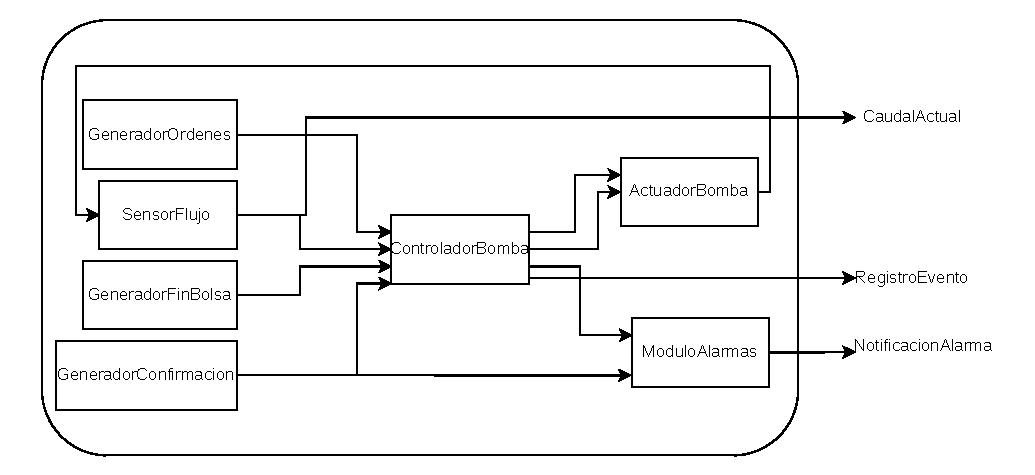
\includegraphics[width=\textwidth]{../Documentacion/diagrama.pdf}
    \caption{Modelo Acoplado del Sistema de Bomba de Infusión}
    \label{fig:acoplado}
\end{figure}

\vspace{1em}

\begin{table}[H]
    \centering
    \caption{Conexiones internas del modelo acoplado}
    \label{tab:conexiones-acoplado}
    \begin{tabularx}{\textwidth}{LL}
        \toprule
        \textbf{Origen} & \textbf{Destino} \\
        \midrule
        \texttt{GeneradorOrdenes.ordenMedica} &
        \texttt{ControladorBomba.ordenMedica} \\
        \texttt{ControladorBomba.ajustarCaudal} &
        \texttt{ActuadorBomba.ajustarCaudal} \\
        \texttt{ControladorBomba.detenerBomba} &
        \texttt{ActuadorBomba.detenerBomba} \\
        \texttt{ActuadorBomba.caudalActual} &
        \texttt{SensorFlujo.caudalActual} \\
        \texttt{SensorFlujo.sensorFlujo} &
        \texttt{ControladorBomba.sensorFlujo} \\
        \texttt{GeneradorFinBolsa.finBolsa} &
        \texttt{ControladorBomba.finBolsa} \\
        \texttt{GeneradorConfirmacion.confirmacion} &
        \texttt{ControladorBomba.confirmacion} \\
        \texttt{GeneradorConfirmacion.confirmacion} &
        \texttt{ModuloAlarmas.confirmacion} \\
        \texttt{ControladorBomba.alarma} &
        \texttt{ModuloAlarmas.alarma} \\
        \bottomrule
    \end{tabularx}
\end{table}

Los puertos de salida externos del modelo acoplado son:

\begin{itemize}
    \item \texttt{caudalActual} --- caudal físico real (del
    \texttt{ActuadorBomba}).
    \item \texttt{registrarEvento} --- log de auditoría (del
    \texttt{ControladorBomba}).
    \item \texttt{notificacionAlarma} --- mensajes de alarma (del
    \texttt{ModuloAlarmas}).
\end{itemize}

% ===================================================================
\section{Implementación en PyPDEVS e infraestructura de validación}
% ===================================================================

\subsection{Arquitectura de la implementación}

Cada modelo atómico se implementa como una subclase de
\texttt{AtomicDEVS} de la biblioteca PyPDEVS.  El estado de cada modelo
se almacena en un diccionario (\texttt{self.state}) y se actualiza en
\texttt{extTransition()} e \texttt{intTransition()} retornando un nuevo
diccionario.  La función de avance temporal \texttt{timeAdvance()}
retorna \texttt{self.state["sigma"]}.

El modelo acoplado \texttt{SistemaBomba} extiende \texttt{CoupledDEVS}
e importa los siete modelos atómicos, conectándolos mediante
\texttt{connectPorts()}.  Los puertos de salida externos
(\texttt{caudalActual}, \texttt{registrarEvento},
\texttt{notificacionAlarma}) permiten observar el comportamiento desde
el exterior de la simulación.

La simulación se ejecuta con el motor \texttt{Simulator} de PyPDEVS en
modo Classic DEVS, con los parámetros de configuración definidos en
\texttt{config.py} y la semilla 42 para los generadores estocásticos.
El tiempo de terminación se configura mediante
\texttt{setTerminationTime()}.

\subsection{Sistema de logging}

Para capturar los eventos durante la simulación se implementó un
\texttt{EventLogger} que almacena tuplas
$(\text{tiempo}, \text{puerto}, \text{valor})$ en una lista
ordenada.  La clase \texttt{TracerEventLogger} integra este logger
con el sistema de \textit{tracing} de PyPDEVS, reemplazando el uso de
\texttt{setVerbose()}.  El tracer se instala mediante:

\begin{lstlisting}
sim.setCustomTracer("logger.event_logger", "TracerEventLogger",
                    [logger, verbose])
\end{lstlisting}

El parámetro \texttt{verbose} controla si los eventos se imprimen
en consola durante la simolución, y el \texttt{EventLogger} se pasa
por referencia para que el verificador pueda acceder a los eventos
una vez finalizada la simulación.

\subsection{Verificador de propiedades (P1--P10)}

El \texttt{VerificadorPropiedades} recorre el \texttt{EventLogger}
post-simulación y verifica 10 propiedades distribuidas en tres
categorías:

\subsubsection*{Safety (P1--P3)}

\begin{itemize}
    \item \textbf{P1 -- Caudal cero}: Si la última orden médica es
    caudal cero, no debe haber \texttt{ajustarCaudal > 0} después.
    \item \textbf{P2 -- Caudal máximo}: Ningún \texttt{ajustarCaudal}
    supera el límite de 200 ml/h.
    \item \textbf{P3 -- Crítica sin confirmación}: Tras una alarma
    crítica, no debe haber \texttt{ajustarCaudal} hasta que llegue
    \texttt{confirmacionEnfermero} o una nueva orden médica.
\end{itemize}

\subsubsection*{Liveness (P4--P6)}

\begin{itemize}
    \item \textbf{P4 -- Orden produce acción}: Toda
    \texttt{ordenMedica} debe generar \texttt{ajustarCaudal} o
    \texttt{detenerBomba} dentro de los 3 segundos posteriores.
    \item \textbf{P5 -- Crítica se repite}: Toda alarma crítica no
    confirmada debe retransmitirse eventualmente.
    \item \textbf{P6 -- Fin de bolsa detiene}: Todo evento
    \texttt{finBolsa} debe ser seguido de \texttt{detenerBomba}.
\end{itemize}

\subsubsection*{Temporalidad (P7--P10)}

\begin{itemize}
    \item \textbf{P7 -- Inicio de infusión}: Toda orden con caudal
    positivo produce un ajuste en menos de 3 segundos.
    \item \textbf{P8 -- Alarma media en 5 segundos}: Un desvío
    sostenido por más de 5 segundos dispara \texttt{alarma = "media"}.
    \item \textbf{P9 -- Fin de bolsa en 60 segundos}: La detención
    por fin de bolsa ocurre dentro de los 60 segundos posteriores.
    \item \textbf{P10 -- Crítica se repite cada 10 segundos}: La
    primera repetición de una crítica no confirmada ocurre a los
    30 segundos y las siguientes cada 10 segundos.
\end{itemize}

Cada propiedad retorna un \texttt{ResultadoVerificacion} con el
estado (cumplida/fallida), un detalle textual y la evidencia
(eventos involucrados).  Las propiedades cuyo antecedente nunca se
activa se consideran verdaderas por vacuidad.

\subsection{Reporte de resultados}

La función \texttt{generar\_reporte()} en
\texttt{verificacion/reporte\_resultados.py} calcula métricas
cuantitativas a partir del \texttt{EventLogger}:

\begin{itemize}
    \item \textbf{Alarmas generadas}: conteo por tipo
    (\texttt{baja}, \texttt{media}, \texttt{critica}).
    \item \textbf{Tiempo de respuesta a desvío}: tiempo promedio
    desde el primer ajuste hasta la alarma media.
    \item \textbf{Tiempo de respuesta a fin de bolsa}: tiempo entre
    \texttt{finBolsa} y \texttt{detenerBomba}.
    \item \textbf{Detenciones preventivas}: cantidad total de
    eventos \texttt{detenerBomba}.
    \item \textbf{Porcentaje de infusión correcta}: proporción del
    tiempo donde el caudal real se encuentra dentro del 10\% del
    objetivo, calculado recorriendo la línea de tiempo combinada de
    órdenes y caudales reales.
\end{itemize}

\subsection{Sistema de gráficos}

La función \texttt{graficar\_escenario()} en
\texttt{graficos/graficar\_resultados.py} genera una figura PNG con
tres subplots:

\begin{enumerate}
    \item \textbf{Caudal objetivo vs caudal real}: tres curvas
    escalón (\texttt{drawstyle='steps-post'}) para órdenes médicas
    (azul), ajustes de caudal (verde) y caudal real (rojo), más
    líneas punteadas verticales para alarmas críticas.
    \item \textbf{Estado de la bomba}: reconstrucción de las fases
    del controlador (\texttt{OCIOSO}, \texttt{INFUNDIENDO},
    \texttt{ALERTA\_BOLSA}, \texttt{MEDIA}, \texttt{CRITICA},
    \texttt{PARADA}) con bandas de colores de fondo.
    \item \textbf{Timeline de eventos}: cada tipo de evento en una
    fila separada con marcadores diferenciados, facilitando la
    lectura visual de la secuencia temporal.
\end{enumerate}

La figura incluye un bloque de texto al pie con los parámetros del
escenario, los resultados de verificación y las métricas del
reporte, permitiendo tener toda la información en una sola imagen.
La imagen se guarda en \texttt{graficos/escenario\_\{num\}\_\{slug\}.png}
con 150 dpi.

\subsection{Integración en \texttt{main.py}}

El punto de entrada \texttt{main.py} coordina todo el flujo:

\begin{enumerate}
    \item Selecciona la configuración del escenario según el
    argumento \texttt{-{}-escenario} (1--9).
    \item Crea un \texttt{EventLogger} y configura el
    \texttt{TracerEventLogger} como tracer personalizado.
    \item Instancia \texttt{SistemaBomba} y \texttt{Simulator},
    ejecuta la simulación en modo Classic DEVS.
    \item Si se especifica \texttt{-{}-verificar} o
    \texttt{-{}-graficos}, ejecuta el \texttt{VerificadorPropiedades}
    y muestra los resultados en consola.
    \item Si se especifica \texttt{-{}-graficos}, genera el PNG con
    \texttt{graficar\_escenario()} incluyendo el reporte de
    métricas.
\end{enumerate}

% ===================================================================
\section{Escenarios de simulación y resultados}
% ===================================================================

\subsection{Escenarios definidos}

Se definieron 9 escenarios que cubren operación normal, condiciones
de falla y una violación deliberada de seguridad.  La
Tabla~\ref{tab:escenarios} resume los parámetros principales.

\begin{table}[ht]
    \centering
    \caption{Resumen de escenarios de simulación}
    \label{tab:escenarios}
    \begin{tabularx}{\textwidth}{cL}
        \toprule
        \textbf{N.} & \textbf{Descripción} \\
        \midrule
        1 & Operación normal: caudal fijo 100 ml/h cada 20 s, sin fallas \\
        2 & Órdenes estocásticas (Gaussiana), sin fallas \\
        3 & Orden única con caudal = 0 (detención programada) \\
        4 & Desvío leve: actuador al 85\% (15\% de desvío), < 5 s \\
        5 & Desvío grave: actuador al 80\% (20\% de desvío), sostenido,
            sin confirmación \\
        6 & Fin de bolsa determinístico en t=30 s, confirmación en t=50 s \\
        7 & Alarma crítica sin confirmación (deriva de sensor) \\
        8 & Fin de bolsa estocástico (Normal) con confirmación
            estocástica (Log-Normal) y ruido en sensor \\
        9 & Violación: mismo desvío que escenario 5 pero con
            \texttt{violar\_seguridad=True} \\
        \bottomrule
    \end{tabularx}
\end{table}

\subsection{Escenarios determinísticos (1--7)}

A continuación se describe cada escenario y su comportamiento esperado.

\paragraph{Escenario 1 -- Operación normal.} El actuador entrega el
caudal exacto de la orden (100 ml/h) cada 20 segundos.  No hay desvío,
no hay fin de bolsa ni alarmas.  El sistema permanece en
\texttt{INFUNDIENDO} todo el tiempo.

\paragraph{Escenario 2 -- Órdenes estocásticas.} El caudal de las
órdenes se muestrea de una Gaussiana $\mathcal{N}(100, 15)$ ml/h y el
interarribo de una Exponencial con media 10 segundos (semilla 42).
El sistema sigue el caudal variable sin desvíos sostenidos.

\paragraph{Escenario 3 -- Orden caudal cero.} Una única orden con
caudal 0 a los 5 segundos.  El controlador emite
\texttt{detenerBomba} y queda en \texttt{OCIOSO}.  Verifica P1.

\paragraph{Escenario 4 -- Desvío leve.} El actuador opera al 85\%
(\texttt{factor\_falla = 0.85}), generando un desvío del 15\%.  La
orden única a los 20 segundos provoca un ajuste; el desvío persiste
menos de 5 segundos antes de que llegue la siguiente orden, por lo
que no se dispara alarma media.

\paragraph{Escenario 5 -- Desvío grave.} El actuador opera al 80\%
(\texttt{factor\_falla = 0.80}), generando un desvío permanente del
20\%.  Sin confirmación del enfermero, el desvío sostenido supera
5 segundos, dispara alarma media, y al acumularse dos episodios de
alarma media sin corrección, escala a alarma crítica, deteniendo la
bomba.

\paragraph{Escenario 6 -- Fin de bolsa.} La bolsa se agota en
t=30 segundos.  El controlador emite alarma baja y permite 60
segundos adicionales de infusión.  En t=50 segundos llega la
confirmación del enfermero; si no hubiera llegado, la bomba se
detendría a los 90 segundos (30 + 60).

\paragraph{Escenario 7 -- Alarma crítica sin confirmación.} Sin
fin de bolsa ni falla en el actuador, la deriva del sensor
(\texttt{TASA\_DERIVA\_SENSOR = 2\%/s}) genera un desvío que escala
a alarma media y luego a crítica.  Sin confirmación, la alarma
crítica se repite cada 30 segundos y luego cada 10 segundos.

\subsection{Escenarios estocásticos (8)}

\paragraph{Escenario 8 -- Fin de bolsa estocástico.} Combina fin de
bolsa con distribución Normal ($\mu=30$, $\sigma=2$), confirmación
Log-Normal ($\mu=2.5$, $\sigma_{\ln}=0.8$), y ruido gaussiano en el
sensor ($\sigma=0.5$).  Evalúa el comportamiento del sistema bajo
variabilidad estadística.

\subsection{Escenario 9 -- Violación deliberada de seguridad}

El escenario 9 replica el escenario 5 (desvío grave) pero
con el flag \texttt{violar\_seguridad\allowbreak=True}.  Esto
desactiva el guarda que impide que el controlador procese
lecturas del sensor durante la fase \texttt{ALARMA\_CRITICA}.
Como consecuencia, tras la detención por alarma crítica, una
nueva lectura del sensor reactiva la infusión, generando un
\texttt{ajustarCaudal} ilegal.  El verificador detecta esta
violación en P3:

\begin{lstlisting}
[X] P3: Safety - critica sin confirmacion
    Ajuste antes de reanudacion en t=50.0
\end{lstlisting}

Las otras 9 propiedades (P1--P10 excepto P3) se cumplen, demostrando
que la violación es quirúrgica y no afecta el resto del sistema.

\subsection{Resultados de verificación}

La Tabla~\ref{tab:matriz-resultados} muestra los resultados de las
10 propiedades para cada escenario.  La simbología sigue la misma
convención de la matriz de cobertura: \checkmark{} para propiedades
cumplidas, \ding{55} para violadas, y --- para verdad vacua.

\begin{table}[ht]
    \centering
    \caption{Resultados de verificación por escenario}
    \label{tab:matriz-resultados}
    \begin{tabular}{lccccccccc}
        \toprule
        \textbf{Prop} & \textbf{1} & \textbf{2} & \textbf{3} & \textbf{4} & \textbf{5} & \textbf{6} & \textbf{7} & \textbf{8} & \textbf{9} \\
        \midrule
        P1 & --- & --- & \checkmark & --- & --- & --- & --- & --- & --- \\
        P2 & \checkmark & \checkmark & \checkmark & \checkmark & \checkmark & \checkmark & \checkmark & \checkmark & \checkmark \\
        P3 & --- & --- & --- & --- & \checkmark & --- & \checkmark & --- & \ding{55} \\
        P4 & \checkmark & \checkmark & \checkmark & \checkmark & \checkmark & \checkmark & \checkmark & \checkmark & \checkmark \\
        P5 & --- & --- & --- & --- & \checkmark & --- & \checkmark & --- & \checkmark \\
        P6 & --- & --- & --- & --- & --- & \checkmark & --- & \checkmark & --- \\
        P7 & \checkmark & \checkmark & --- & \checkmark & \checkmark & \checkmark & \checkmark & \checkmark & \checkmark \\
        P8 & --- & --- & --- & \checkmark & \checkmark & --- & \checkmark & --- & \checkmark \\
        P9 & --- & --- & --- & --- & --- & \checkmark & --- & \checkmark & --- \\
        P10 & --- & --- & --- & --- & \checkmark & --- & \checkmark & --- & \checkmark \\
        \bottomrule
    \end{tabular}
\end{table}

\subsection{Análisis de resultados}

Los resultados confirman que:

\begin{itemize}
    \item \textbf{Todas las propiedades tienen cobertura}: cada
    propiedad tiene al menos un escenario donde su antecedente se
    activa y el consecuente se evalúa realmente.  No hay propiedades
    siempre vacuas.

    \item \textbf{Solo P3 falla en el escenario 9}: la violación
    deliberada de seguridad demuestra que el verificador detecta
    correctamente el comportamiento indebido.  Las 9 propiedades
    restantes se cumplen incluso en este escenario, lo que indica que
    la violación es localizada.

    \item \textbf{P2, P4 y P7 son ubicuas}: se activan en casi todos
    los escenarios porque no requieren condiciones especiales (ajustes
    y órdenes existen en prácticamente todos los casos).

    \item \textbf{P6 y P9 son las más específicas}: solo se activan
    en escenarios con evento de fin de bolsa (6 y 8).
\end{itemize}

\subsection{Reporte de métricas}

Para cada escenario se calculan métricas cuantitativas que permiten
evaluar el rendimiento del sistema:

\begin{itemize}
    \item \textbf{Alarmas generadas}: el escenario 5 (desvío grave sin
    confirmación) genera 6 alarmas (2 medias, 4 críticas).  El
    escenario 9 (violación) genera 16 alarmas (2 medias, 14 críticas)
    porque la violación reinicia el ciclo de desvío repetidamente.

    \item \textbf{Tiempo de respuesta a desvío}: en los escenarios
    con desvío sostenido (4, 5, 7, 9), la alarma media se dispara
    aproximadamente 5 segundos después del primer ajuste, cumpliendo
    el requisito temporal.

    \item \textbf{Detenciones preventivas}: el escenario 5 presenta
    4 detenciones y el escenario 9 presenta 14 detenciones, reflejo
    del reinicio continuo del ciclo de alarma crítica.

    \item \textbf{Porcentaje de infusión correcta}: en los escenarios
    sin falla (1, 2, 3) el porcentaje es cercano al 100\%.  En
    escenarios con desvío permanente (5, 9) el porcentaje es 0\%
    porque nunca se alcanza el caudal objetivo.  En el escenario 6
    (fin de bolsa con confirmación) el porcentaje se mantiene alto
    porque la infusión se detiene ordenadamente.
\end{itemize}

\subsection{Análisis visual}

Los gráficos generados para cada escenario (Figura~\ref{fig:ejemplo-grafico})
permiten visualizar simultáneamente:

\begin{enumerate}
    \item La evolución del caudal objetivo, los ajustes y el caudal
    real (curvas escalón), con líneas punteadas verticales para
    alarmas críticas.
    \item Las fases del controlador (\texttt{OCIOSO},
    \texttt{INFUNDIENDO}, \texttt{ALERTA\_BOLSA}, \texttt{MEDIA},
    \texttt{CRITICA}, \texttt{PARADA}) con bandas de colores.
    \item El timeline de eventos con marcadores diferenciados para
    cada tipo de evento (órdenes, ajustes, alarmas, confirmaciones,
    fin de bolsa, detenciones).
\end{enumerate}

Cada PNG incluye al pie los parámetros del escenario, el resultado
de la verificación y las métricas del reporte, ofreciendo una
visualización completa del comportamiento del sistema.

\begin{figure}[H]
    \centering
    \includegraphics[width=\textwidth]{../graficos/escenario_5_desvio_grave.png}
    \caption{Ejemplo de gráfico generado: escenario 5 (desvío grave)}
    \label{fig:ejemplo-grafico}
\end{figure}

% ===================================================================
\section{Mejoras propuestas}
% ===================================================================

A partir del análisis de los resultados de simulación y verificación,
se identificaron dos áreas de mejora para reducir riesgos en el
controlador de la bomba de infusión.

\subsection{Rate limiting en ajustes de caudal}

\paragraph{Problema identificado.}  En la implementación actual,
cuando el sensor detecta un desvío sostenido, el controlador puede
emitir ajustes de caudal en cada ciclo del sensor (cada 1 segundo)
mediante la expresión:

\[
\sigma = \min(\sigma_{\text{restante}},\;
              \sigma_{\min}(t_{\text{desvío}}, t_{\text{bolsa}}))
\]

Cuando \(\sigma_{\text{restante}} \approx 1.0\) (próxima transición
interna del controlador, que coincide aproximadamente con el período
del sensor) y \(t_{\text{desvío}} > 0\), el sigma resultante es
\(\approx 1.0\), generando un ajuste cada segundo.  Sin embargo, el
actuador tiene una latencia física de 0.5 segundos
(\texttt{LATENCIA\_ACTUADOR}) para aplicar cada cambio.  Si el
controlador emite un nuevo ajuste antes de que el actuador haya
completado el anterior, se producen dos problemas:

\begin{enumerate}
    \item \textbf{Oscilaciones}: el controlador corrige sobre un valor
    que aún no se ha materializado, pudiendo sobrepasar el objetivo.
    \item \textbf{Ineficiencia}: el actuador recibe más comandos de
    los que puede procesar, desperdiciando ciclos de simulación.
\end{enumerate}

\paragraph{Propuesta.}  Agregar una constante
\texttt{MIN\_INTERVALO\_AJUSTE = 0.5} (igual a la latencia del
actuador) y modificar la lógica de sigma en desvío sostenido para
que el controlador no emita ajustes con una frecuencia mayor a la
que el actuador puede responder:

\[
\sigma = \min\bigl(\max(\sigma_{\text{restante}},
                        \texttt{MIN\_INTERVALO\_AJUSTE}),\;
                  \sigma_{\min}(t_{\text{desvío}}, t_{\text{bolsa}})\bigr)
\]

\paragraph{Impacto esperado.}
\begin{itemize}
    \item Menor cantidad de eventos \texttt{ajustarCaudal}.
    \item Curva de caudal real más estable (menos oscilaciones).
    \item El porcentaje de tiempo con infusión correcta se mantiene
    o mejora porque los ajustes son más efectivos.
\end{itemize}

\subsection{Watchdog de sensor}

\paragraph{Problema identificado.}  El sistema asume que el sensor de
flujo siempre reporta lecturas cada \texttt{PERIODO\_SENSOR = 1.0}
segundos, pero no hay ningún mecanismo que verifique que el sensor
está funcionando correctamente.  Si el sensor falla (se desconecta,
se rompe, o el cable se daña):

\begin{enumerate}
    \item El controlador nunca recibe eventos \texttt{sensorFlujo}.
    \item Permanece en la última fase en la que estaba.
    \item Si estaba en \texttt{INFUNDIENDO} y no hay desvío, sigue
    infundiendo indefinidamente sin supervisión.
    \item Si el caudal real se desvía (obstrucción parcial o falla
    del actuador), el controlador no lo detecta por falta de
    mediciones.
\end{enumerate}

Esto constituye un riesgo de seguridad grave: la bomba puede estar
entregando un caudal incorrecto sin que el sistema lo sepa.

\paragraph{Propuesta.}  Agregar un \textbf{watchdog timer} al estado
del controlador que detecte la ausencia de lecturas del sensor:

\begin{itemize}
    \item El controlador lleva la cuenta del tiempo desde la última
    lectura del sensor en \(t_{\text{ultimoSensor}}\).
    \item En cada \texttt{intTransition}, incrementa
    \(t_{\text{ultimoSensor}}\) por \(\sigma\).
    \item Si \(t_{\text{ultimoSensor}} > 2 \times
    \texttt{PERIODO\_SENSOR} = 2.0\) segundos, se considera que el
    sensor falló y se entra en un estado \texttt{FALLA\_SENSOR}.
    \item En \texttt{FALLA\_SENSOR}, se emite \texttt{alarmaCritica},
    \texttt{detenerBomba}, y se queda pasivo hasta recibir
    confirmación.
    \item Al recibir una nueva lectura del sensor (\texttt{sensorFlujo}
    en \texttt{extTransition}), se resetea
    \(t_{\text{ultimoSensor}} = 0\) y se sale de
    \texttt{FALLA\_SENSOR}.
\end{itemize}

\paragraph{Escenario de prueba propuesto.}  Se podría crear un
\texttt{escenario 10: falla de sensor} donde el \texttt{SensorFlujo}
deje de emitir después de cierto tiempo.  A los 2 segundos sin
lecturas, el controlador debe entrar en \texttt{FALLA\_SENSOR},
emitir alarma crítica y detener la bomba.  Se agregaría una propiedad
\texttt{P11}: \textit{si el sensor deja de reportar por más de 2
segundos, se debe emitir alarma crítica y detener la bomba}.

% ===================================================================
\section{Conclusiones}
% ===================================================================

En este trabajo se presentó el modelado, la implementación y la
verificación de un controlador para bomba de infusión intravenosa
utilizando el formalismo DEVS y la herramienta PyPDEVS.  El sistema
fue especificado mediante siete modelos atómicos DEVS que representan
los componentes físicos y lógicos de la bomba, integrados en un modelo
acoplado que reproduce el comportamiento del sistema real.

Se diseñaron nueve escenarios de simulación que cubren operación
normal, condiciones de falla (desvío de caudal, fin de bolsa, deriva
de sensor) y una violación deliberada de seguridad.  Para cada
escenario se ejecutaron diez verificaciones de propiedades (P1--P10)
que abarcan requisitos de seguridad, correcto funcionamiento y
temporales.  Todas las propiedades se cumplen en los escenarios
nominales y de falla; únicamente la propiedad P3 falla en el
escenario 9 (violación deliberada), demostrando que el verificador
detecta correctamente el comportamiento indebido.

La infraestructura de validación desarrollada --- compuesta por un
registrador de eventos, un verificador de propiedades, un generador
de reportes de métricas y un visualizador gráfico --- demostró ser
eficaz para evaluar el comportamiento del sistema de forma
sistemática.  La matriz de cobertura confirma que cada propiedad tiene
al menos un escenario donde su antecedente se activa, lo que garantiza
que ninguna propiedad es siempre vacua.

El modelado estocástico de órdenes médicas, fin de bolsa,
confirmaciones y ruido del sensor permitió evaluar la robustez del
sistema bajo condiciones de incertidumbre.  La inclusión de semillas
fijas (seed = 42) asegura la reproducibilidad de los resultados.

Entre las limitaciones del trabajo se encuentra la ausencia de un
mecanismo de watchdog para detectar fallas del sensor y la falta de
rate-limiting en los ajustes de caudal, aspectos que quedan como
trabajo futuro.  Asimismo, la separación del puerto único de alarmas
en tres puertos diferenciados (baja, media, crítica) mejoraría la
modularidad del modelo.

En conclusión, el enfoque basado en DEVS con verificación formal de
propiedades resultó adecuado para modelar y validar un sistema de
control de infusión intravenosa, demostrando que es posible detectar
automáticamente violaciones de seguridad y garantizar el cumplimiento
de requisitos críticos en un sistema de software para salud.

\end{document}
